\chapter{Used data}

There was one main criterion when choosing a dataset for this data. It needed enough features ($> 256$) for images transformed by REFINED to make sense. Based on this requirement, an excellent data source has presented itself as data created by P2Rank - a software offered by \cite{P2RANK}. In this chapter, I'll first explain in detail the origin of the data, including the chemical background, the importance of the problem in the real world, and the precise way the data was created. Then, I'll explain this dataset from a data science or machine learning point of view, with all relevant information included. 

\section{Chemical view on datasets}
\begin{figure}
    \centering
    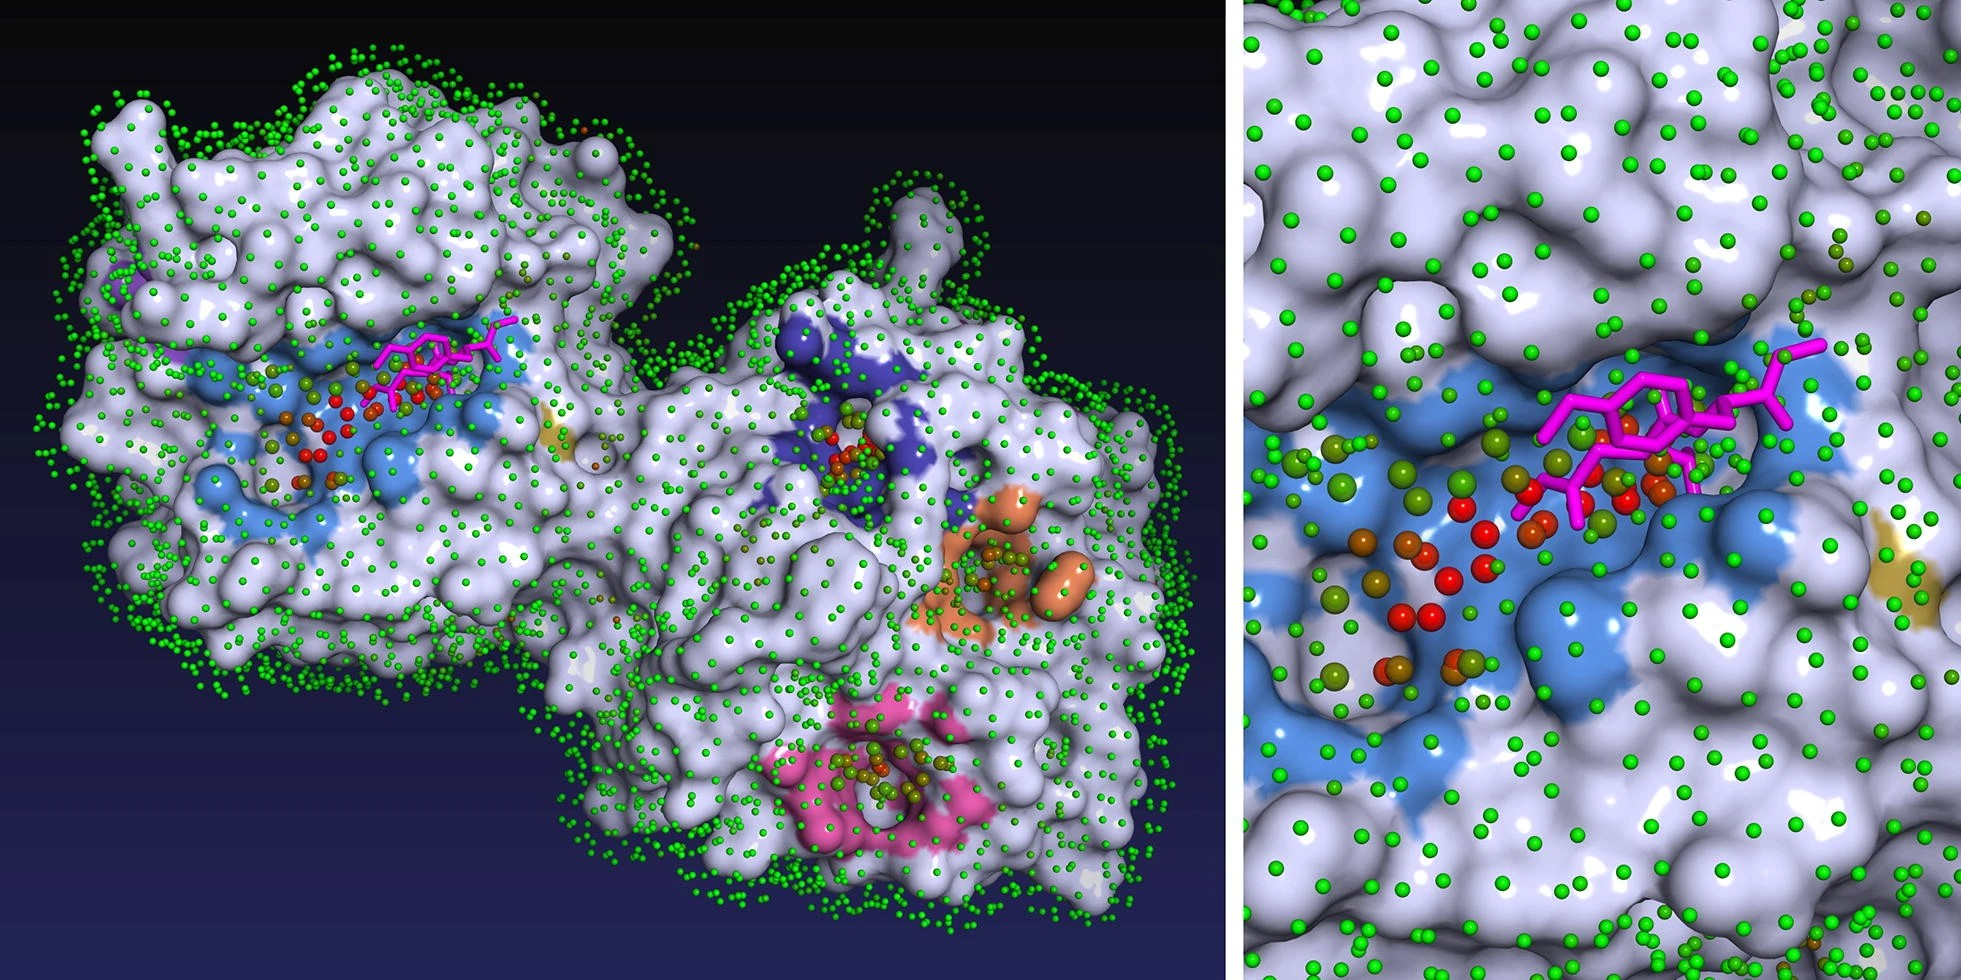
\includegraphics[width=1\linewidth]{p2rank.jpg}
    \caption{Visualization of a molecule taken directly from \cite{P2RANK}. The protein surface is covered by SAS points represented by green to red points representing predicted ligandability  (from 0 = green to 1 = red). The largest pocket (shown in the close-up) is indeed a correctly predicted true binding site that binds a known ligand (magenta). }
    \label{fig:p2rank_visualization}
\end{figure}
% https://jcheminf.biomedcentral.com/articles/10.1186/s13321-018-0285-8#Sec1
\textit{Ligand Binding Sites} (LBS) prediction from protein structure is an important part of biochemistry needed for...

\subsection{Protein structure}

Proteins are organic macromolecules. They are long chains of smaller molecules called amino acids, and there are hundreds in a chain.

An amino acid is a small molecule containing an amino group (N-terminus) and a carboxyl group (C-terminus). In a protein, individual amino acids are connected by a peptide bond that connects these two groups of adjacent amino acids.

// pořadí aminokyselin - primární struktura
// sek.struktura
// pro LBS je zásadní struktura terciární.

The instructions for making a protein are stored in DNA. Transcribing the genetic code produces mRNA, which serves as a template for the protein. Ribosome units are mounted on this template, and with their help, the individual amino acids forming the protein are connected. As the protein exits the ribosome, folding occurs to ensure the correct 3D structure of the protein. Larger proteins do not fold independently but need auxiliary proteins, so-called chaperones, to fold correctly. The resulting structure is essential for the protein's biological activity and can be used to predict the ligandability of a substance.

The LBS model, therefore, works with the protein's 3D structure and examines whether the given ligand can bind in such a place or whether the protein's surface is unsuitable for binding.

% Tk. Cite: Autor 	Kodíček Milan, Valentová Olga, Hynek Radovan
% Vydavatel 	VŠCHT Praha (3. vydání, 2022)
% ISBN 	978-80-7592-124-6


\subsection{Ligand Binding Sites}

Ligand binding sites are parts of the protein's surface where a bond with some ligand can be created. Ligand can be another protein, for instance, a receptor or enzyme. However, the precise definition differs per dataset. Prediction of these binding sites is useful in computer-aided drug design, and it is being used to analyze and compare all known and putative binding sites on a genome-wide level \cite{P2RANK}.

Other use cases are...



\section{Data science view on datasets}

With the dataset creation understood from the real-world side, let us now look at how it is handled from a machine-learning point of view. 

\subsection{Raw data intuition}

The raw input into any of our models is the protein's 3D structure. This is represented by a point cloud on the protein's surface. Each point has a feature vector attached, which represents the chemical properties of the given accessible surface patch. Each point also has an LBS class, which the model trains and predicts. These can be seen in the figure~\ref{fig:data_point_cloud}.

\begin{figure}
    \centering
    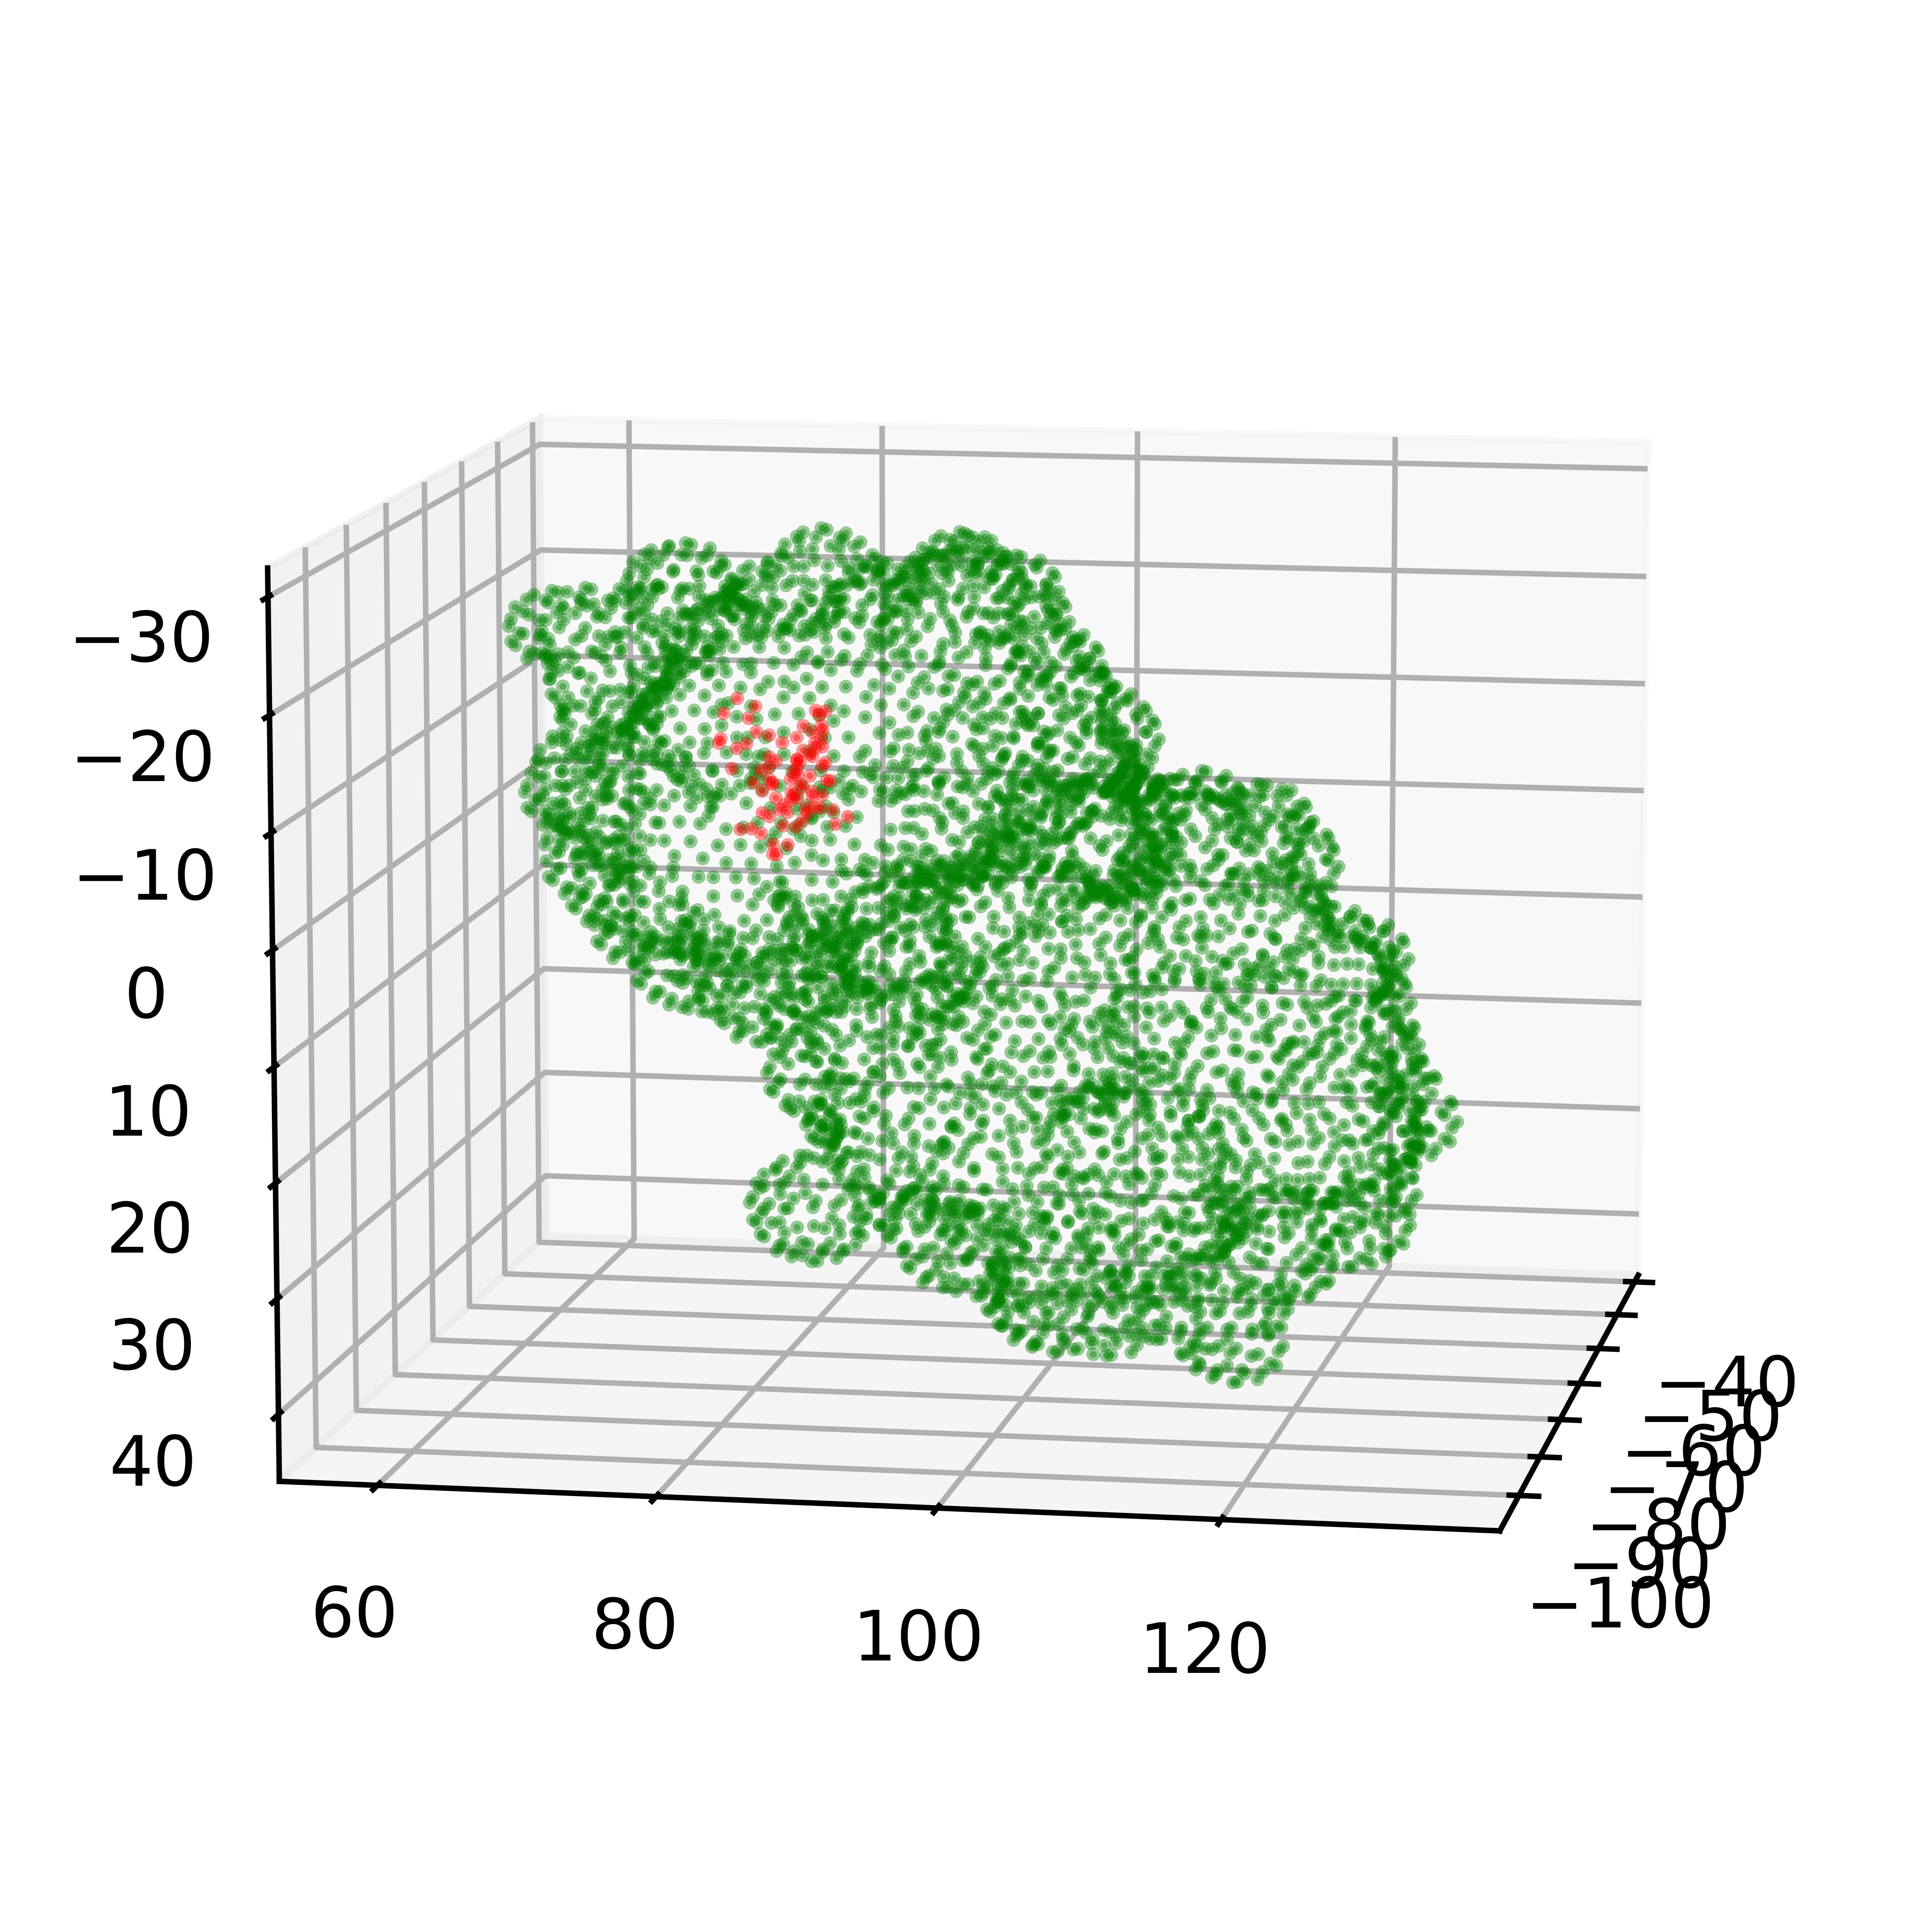
\includegraphics[width=1\linewidth]{point_cloud_class.png}
    \caption{SAS point cloud representing a protein with a highlighted ligand-binding site (in red). This point cloud is the input into the whole pipeline discussed in this work. Compare it to the P2Rank visualization in ~\ref{fig:p2rank_visualization} and feature visualization in }
    \label{fig:pca_point_cloud}. This visualization was created by matplotlib.pyplot.scatter3D.
\end{figure}

\begin{figure}
    \centering
    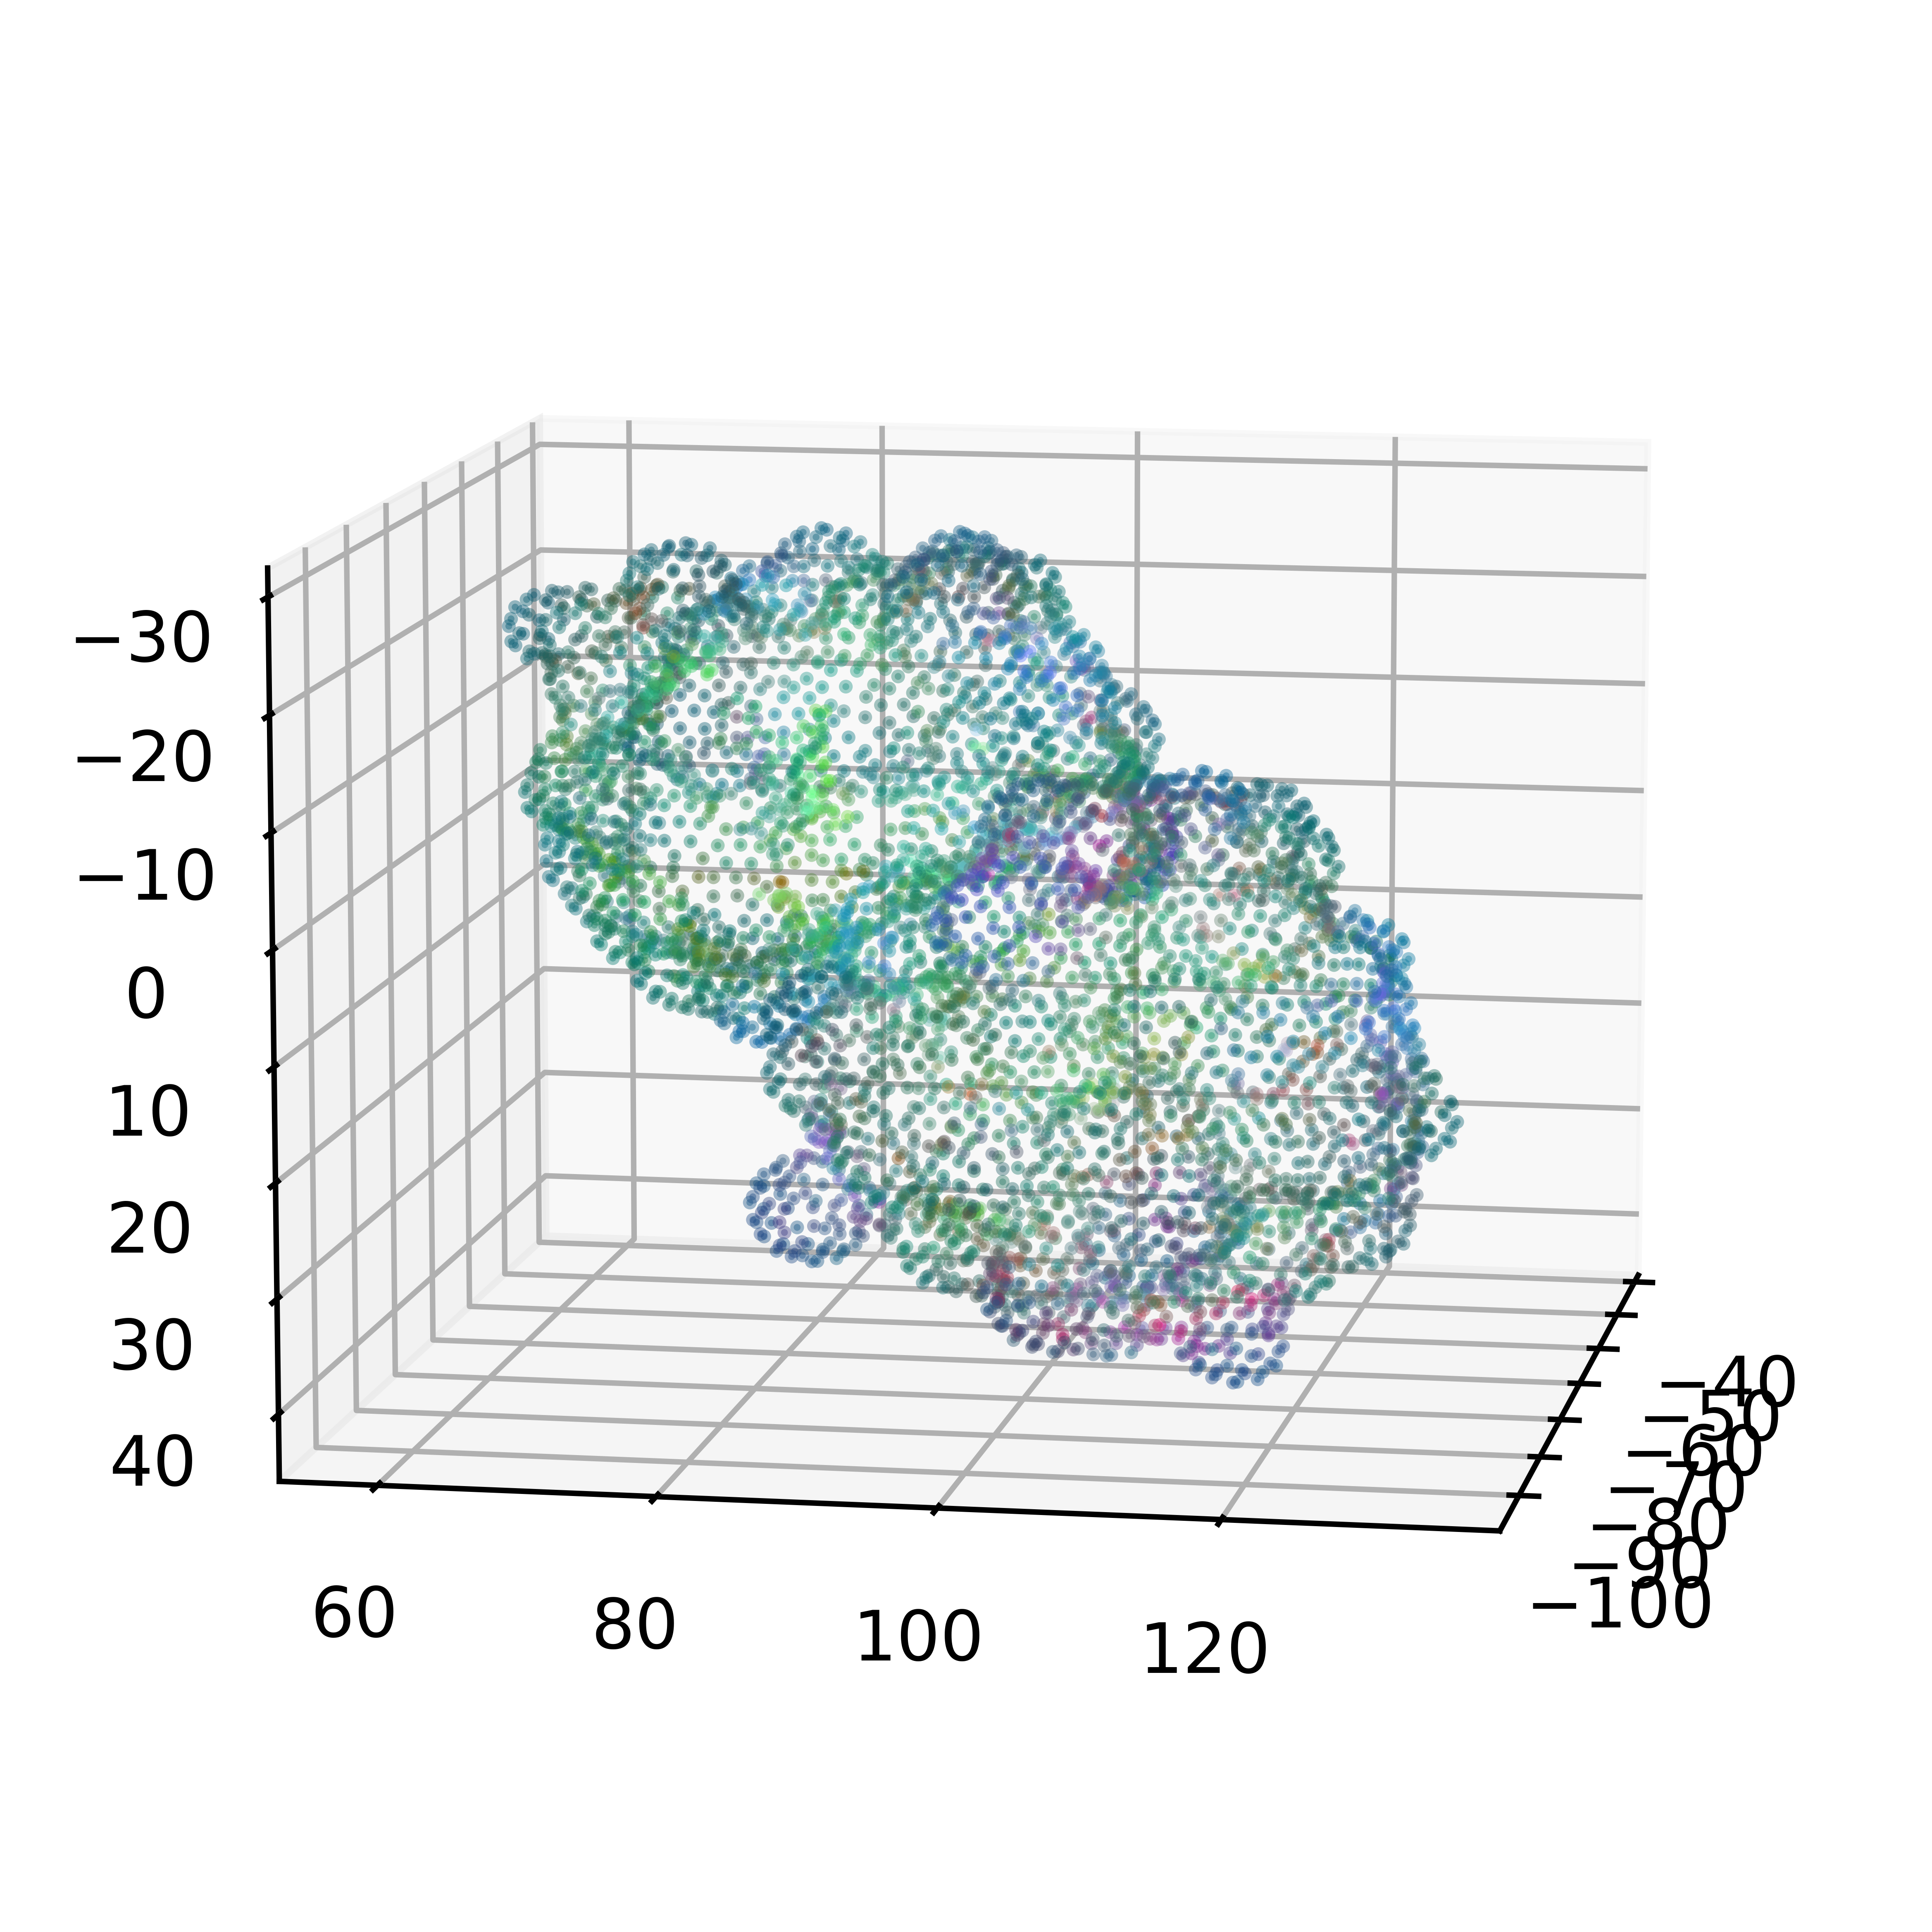
\includegraphics[width=1\linewidth]{point_cloud_pca.png}
    \caption{SAS point cloud showing the distribution of features across the surface. To achieve this visualization, locational and class-defining features were removed. Scikit-learn's PCA then reduced the remaining 35 dimensions to 3 dimensions. These were then plotted as red, green and blue channels using matplotlib.pyplot.scatter3D. It can be seen that there are no major feature outliers in the LBS area.}
    \label{fig:pca_point_cloud}
\end{figure}

In the implementation, these points are represented as tabular data, with three columns representing the X, Y, and Z axis, respectively. From this data, the point cloud can be recreated.

\subsection{Ligand-binding sites}

LBS represent protein parts, where a ligand (another chemically active substance) can bond to the protein. In \textit{chen11} and \textit{coach420} datasets, the ligand can be any chemical substance passing some essential criteria. These limit the size (not too small, not too big) and chemical bond type (for example, ions are excluded, as these use a different mechanism of chemical bond). In the \textit{ATP} dataset, only ATP (\textbf{A}denosine \textbf{T}ri\textbf{p}hosphate) is considered as a possible ligand. (Tk: add other datasets).

Clusters of points represent LBS in our data. There is usually one LBS per protein, but more can also exist. In some cases, no LBS is in the whole protein (but most of these proteins have been filtered out during the data preprocessing).

\subsection{Features}

As mentioned above, each point from the cloud has a feature vector attached. These features are fully described in [TK: attachment]. The exact features are essential for result reproducibility. However, they are not important for understanding these experiments. 

These features represent chemical properties of the protein surface (such as hydrophobicity), surface shape (protrusion), or physical properties (XYZ coordinates). All of them represent a float value and are used as such - no binary or class features are used (atomic number could be seen as a class feature, but similarly sized atoms will have some similarities in their properties, so this feature is used as a numeric one as well).

\subsection{Surroundings extraction}
\label{Surroundings}

As described in the previous chapter, for the proposed algorithm to work, we need to have more features.

To achieve this, we run the following algorithm to extract the surroundings (some parts were simplified compared to the actual code by omitting performance improvements and ignoring some syntactical parts for the reasons of readability):

\begin{lstlisting}
def extract_surroundings(protein: pd.DataFrame, size: int, labels: pd.Series) -> np.array:
  surroundings_dataset = []
  for i in range(len(protein)):
    surroundings_datasetFor.append(
      protein.sort(
          key = lambda x: mahattan_distance(i, x)
            )[:size].flatten()
      )
  return surroundings_dataset, labels
\end{lstlisting}

Or, in natural language, for each point in the original protein surface, we take the $k$ nearest points to the original point. All features from these points are then concatenated, and labels are kept from the original data.

Having a larger context naturally improves the performance of any model. In \cite{P2RANK}, proposing this dataset, a larger context area is not considered in the models themselves but as a postprocessing step, where clusters of positively predicted points identify LBS.

This way of creating the dataset has another advantage. SAS points that are close to each other often have highly correlated features. This, in turn, should help the REFINED algorithm even further.

Tk: Add a graphics showing this process

Tk: move to discussion.
This algorithm is not asymptotically optimal, as it calculates the surroundings in $O(n^2 \log{n})$, where $n$ is the number of points from the protein. Using a structure such as a \textit{k-d tree} (proposed by \cite{kd-tree}), this can be trivially reduced to $O(n \log{n})$. 